% 在原图上仅覆盖自然语言文字区域，保留全部图标、面板、对话框边框及数据含义。
\begingroup
\linespread{1}\selectfont
\definecolor{ch13MedPink}{RGB}{247,214,207}
\definecolor{ch13MedGreen}{RGB}{229,240,219}
\definecolor{ch13MedYellow}{RGB}{253,242,208}
\definecolor{ch13MedGray}{RGB}{237,237,237}
\newlength{\chThirteenMedUnit}
\setlength{\chThirteenMedUnit}{\dimexpr\linewidth/1748\relax}
\newcommand{\chThirteenMedBlock}[7]{%
  \fill[#5] (#1,#2) rectangle (#3,#4);
  \node[inner sep=0pt,align=left,
    text width=\dimexpr#3\chThirteenMedUnit-#1\chThirteenMedUnit-12\chThirteenMedUnit\relax,
    font=#6] at ({(#1+#3)/2},{(#2+#4)/2}) {#7};
}
\begin{tikzpicture}[x=\chThirteenMedUnit,y=-\chThirteenMedUnit]
  \node[anchor=north west,inner sep=0pt] at (0,0) {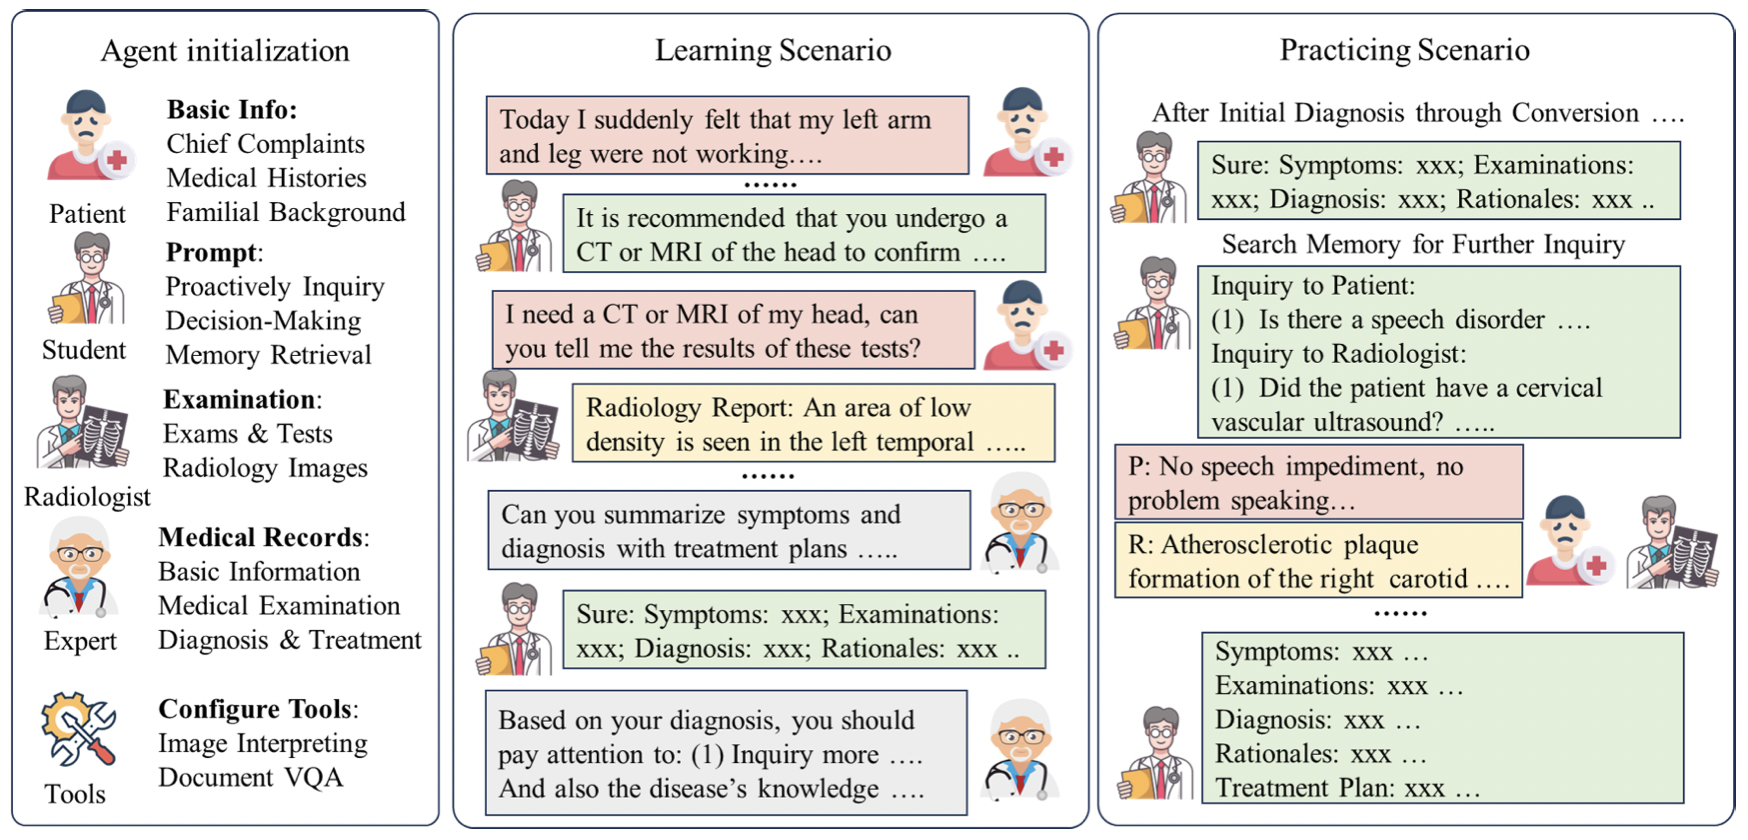
\includegraphics[width=\linewidth]{figures/medco.png}};
  % 智能体初始化面板：原有角色和全部字段。
  \fill[white] (55,28) rectangle (414,75);
  \node[font=\fontsize{9}{11}\selectfont\bfseries] at (234,51) {智能体初始化};
  \chThirteenMedBlock{20}{199}{151}{229}{white}{\fontsize{8.2}{10}\selectfont}{\centering 患者}
  \chThirteenMedBlock{20}{334}{151}{366}{white}{\fontsize{8.2}{10}\selectfont}{\centering 学生}
  \chThirteenMedBlock{13}{480}{154}{512}{white}{\fontsize{8}{9}\selectfont}{\centering 放射医师}
  \chThirteenMedBlock{24}{626}{143}{660}{white}{\fontsize{8.2}{10}\selectfont}{\centering 专家}
  \chThirteenMedBlock{23}{782}{143}{815}{white}{\fontsize{8.2}{10}\selectfont}{\centering 工具}
  \chThirteenMedBlock{157}{88}{431}{229}{white}{\fontsize{7.6}{8.5}\selectfont}
    {\textbf{基本信息：}\\主诉\\病史\\家庭背景}
  \chThirteenMedBlock{157}{238}{431}{369}{white}{\fontsize{7.6}{8.5}\selectfont}
    {\textbf{提示：}\\主动问诊\\决策\\记忆检索}
  \chThirteenMedBlock{154}{380}{431}{492}{white}{\fontsize{7.6}{8.5}\selectfont}
    {\textbf{检查：}\\查体与检验\\放射影像}
  \chThirteenMedBlock{153}{521}{431}{655}{white}{\fontsize{7.6}{8.5}\selectfont}
    {\textbf{医疗记录：}\\基本信息\\医学检查\\诊断与治疗}
  \chThirteenMedBlock{152}{695}{431}{796}{white}{\fontsize{7.6}{8.5}\selectfont}
    {\textbf{配置工具：}\\图像解读\\文档视觉问答}
  % 学习场景：对话次序、说话者图标及省略号原位保留。
  \fill[white] (589,28) rectangle (1037,75);
  \node[font=\fontsize{9}{11}\selectfont\bfseries] at (774,51) {学习场景};
  \chThirteenMedBlock{490}{100}{966}{171}{ch13MedPink}{\fontsize{8}{9.8}\selectfont}
    {今天我突然觉得左臂和左腿\\都不听使唤了……}
  \chThirteenMedBlock{566}{198}{1042}{269}{ch13MedGreen}{\fontsize{8}{9.8}\selectfont}
    {建议你接受头部 CT 或 MRI\\检查，以便确认……}
  \chThirteenMedBlock{496}{295}{972}{367}{ch13MedPink}{\fontsize{8}{9.8}\selectfont}
    {我需要头部 CT 或 MRI 检查，\\能告诉我这些检查的结果吗？}
  \chThirteenMedBlock{576}{387}{1052}{459}{ch13MedYellow}{\fontsize{8}{9.8}\selectfont}
    {放射学报告：左侧颞部\\可见低密度区域……}
  \chThirteenMedBlock{492}{495}{966}{566}{ch13MedGray}{\fontsize{8}{9.8}\selectfont}
    {你能总结症状与诊断，\\并给出治疗方案吗……}
  \chThirteenMedBlock{566}{595}{1042}{665}{ch13MedGreen}{\fontsize{7.8}{9.4}\selectfont}
    {好的：症状：xxx；检查：xxx；\\诊断：xxx；依据：xxx……}
  \chThirteenMedBlock{490}{695}{963}{812}{ch13MedGray}{\fontsize{8}{9.8}\selectfont}
    {根据你的诊断，你应该注意：\\(1) 进一步问诊……\\还要注意有关疾病的知识……}
  % 练习场景：问诊、记忆检索、患者与放射科医师反馈及最终总结。
  \fill[white] (1213,28) rectangle (1694,75);
  \node[font=\fontsize{9}{11}\selectfont\bfseries] at (1417,51) {练习场景};
  \chThirteenMedBlock{1144}{94}{1696}{129}{white}{\fontsize{8.2}{10}\selectfont}
    {\centering 通过对话完成初步诊断后……}
  \chThirteenMedBlock{1202}{146}{1677}{216}{ch13MedGreen}{\fontsize{7.8}{9.4}\selectfont}
    {好的：症状：xxx；检查：xxx；\\诊断：xxx；依据：xxx……}
  \chThirteenMedBlock{1204}{226}{1704}{263}{white}{\fontsize{8.2}{10}\selectfont}
    {\centering 检索记忆，进一步问诊}
  \chThirteenMedBlock{1202}{270}{1677}{435}{ch13MedGreen}{\fontsize{7.8}{8.5}\selectfont}
    {询问患者：\\(1) 是否存在言语障碍……\\询问放射科医师：\\(1) 患者做过颈部血管\\超声检查吗？……}
  \chThirteenMedBlock{1120}{449}{1518}{517}{ch13MedPink}{\fontsize{7.8}{9}\selectfont}
    {P：没有言语障碍，\\说话没有问题……}
  \chThirteenMedBlock{1120}{527}{1518}{594}{ch13MedYellow}{\fontsize{7.8}{9}\selectfont}
    {R：右侧颈动脉有\\粥样硬化斑块形成……}
  \chThirteenMedBlock{1206}{637}{1680}{799}{ch13MedGreen}{\fontsize{7.8}{8.4}\selectfont}
    {症状：xxx……\\检查：xxx……\\诊断：xxx……\\依据：xxx……\\治疗方案：xxx……}
\end{tikzpicture}
\endgroup
